\chapter{GDSE Sensitivity Studies}\label{ch:sensitivity}

The modeling paradigm with which this repository model and simulation 
platform are implemented are described here. 
Sensitivity studies performed with the \gls{GDSM} tools developed within
the national lab system are here described. The results were analyzed to 
capture the salient parameters of readionuclide sequestration in 
various repository geologies.


\subsection{Solubility Coefficients}

This study varied the solubility coefficients for each isotope in the simulation 
to help inform the effect of reprocessing on repository benefit for the clay 
repository scenario. The importance of the actinide contribution relative to the 
contribution from $^{129}I$, $^{79}Se$, and $^{99}Tc$ was of particular 
interest.

The dissolution behavior of a solute in an aqueous solutions is called its 
solubility. This behavior is limited by the solute's solubility limit, described  
by an equilibrium constant that depends upon temperature, water chemistry, and 
the properties of the element. The solubility constant for ordinary solutes, 
$K_s$ gives units of concentration, $[kg/m^3]$, and can be determined 
algebraically by the law of mass action which gives the partitioning at 
equilibrium between reactants and products.  For a reaction
\begin{align}
  cC + dD &= yY + zZ,
  \intertext{where}
  c,d,y,z  &= \mbox{ amount of respective constituent }[mol]\nonumber\\
  C,D  &= \mbox{ reactants }[-]\nonumber\\
  Y,Z  &= \mbox{ products }[-]\nonumber,
  \intertext{the law of mass action gives}
  K &= \frac{(Y)^y(Z)^z}{(C)^c(D)^d}
  \intertext{where}
  (X)  &= \mbox{ the equilibrium molal concentration of X }[mol/m^3]\nonumber\\
  K  &= \mbox{ the equilibrium constant }[-].\nonumber
  \label{massaction}
\end{align}
The equilibrium constant for many reactions are known, and can be found in 
chemical tables. Thereafter, the solubility constraints of a solution at 
equilibrium can be found algebraically.  In cases of salts that  dissociate in 
aqueous solutions, this equilibrium constant is called the salt's solubility 
product $K_{sp}$.

This equilibrium model, however, is only appropriate for dilute situations, and 
nondilute solutions at  partial equilibrium must be treated with an activity 
model by substituting the activities of the constituents  for their molal 
concentrations,
\begin{align}
  [X] &= \gamma_x(X)
  \intertext{where}
  [X]  &= \mbox{ activity of X }[-]\nonumber\\
  \gamma_x  &= \mbox{ activity coefficient of X}[-]\nonumber\\
  (X)  &= \mbox{ molal concentration of X}[mol/m^3]\nonumber
  \intertext{such that}
  IAP &= \mbox{ Ion Activity Product }[-].\nonumber\\
      &= \frac{[Y]^y[Z]^z}{[C]^c[D]^d}\\
  \label{IAP}
\end{align}
The ratio between the IAP and the equilibrium constant $(IAP/K)$ quantifiesn
the departure from equilibrium of a solution.  This information is useful during 
the transient stage in which a solute is first introduced to a solution. When 
$IAP/K<1$, the solution is undersaturated with respect to the products. When, 
conversely, $IAP/K>1$, the solution is oversaturated and precipitation of solids 
in the volume will occur. 

\subsubsection{Parametric Range}

The solubility coefficients were varied in this simulation using a multiplier. 
The reference solubilities for each element were multiplied by the multiplier 
for each simulation group. This technique preserved relative solubility among 
  elements. Forty values of solubility coefficient multiplier were used to change 
the far field solubility. This did not alter any of the solubility in the
EDZ, WF, or Fast Path solubilities.

The values of the solubility multiplier were deliberately varied over many 
magnitudes, from $1\time10^{-9}$ through $5\times10^{10}$. This multiplier
multiplied the most likely values of solubility for each element, so 
the relative solubility between elements was preserved.


\subsubsection{Results}

The results for varying the solubility coefficient were very straightforward.  
For solubility limits below a certain threshold, the dose releases were directly 
proportional to the solubility limit, indicating that the radionuclide 
concentration saturated the groundwater up to the solubility limit near the 
waste form.  For solubility limits above the threshold, however, further 
increase to the limit had no effect on the peak dose. This demonstrates the 
situation in which the solubility limit is so high that even complete 
dissolution of the waste inventory into the pore water is insufficient to reach 
the solubility limit.

In Figures \ref{fig:SolSumFactor} and \ref{fig:SolSum}, it is clear that for 
solubility constants lower than a threshold, the relationship between peak 
annual dose and solubility limit is strong.

\begin{figure}[ht]
\centering
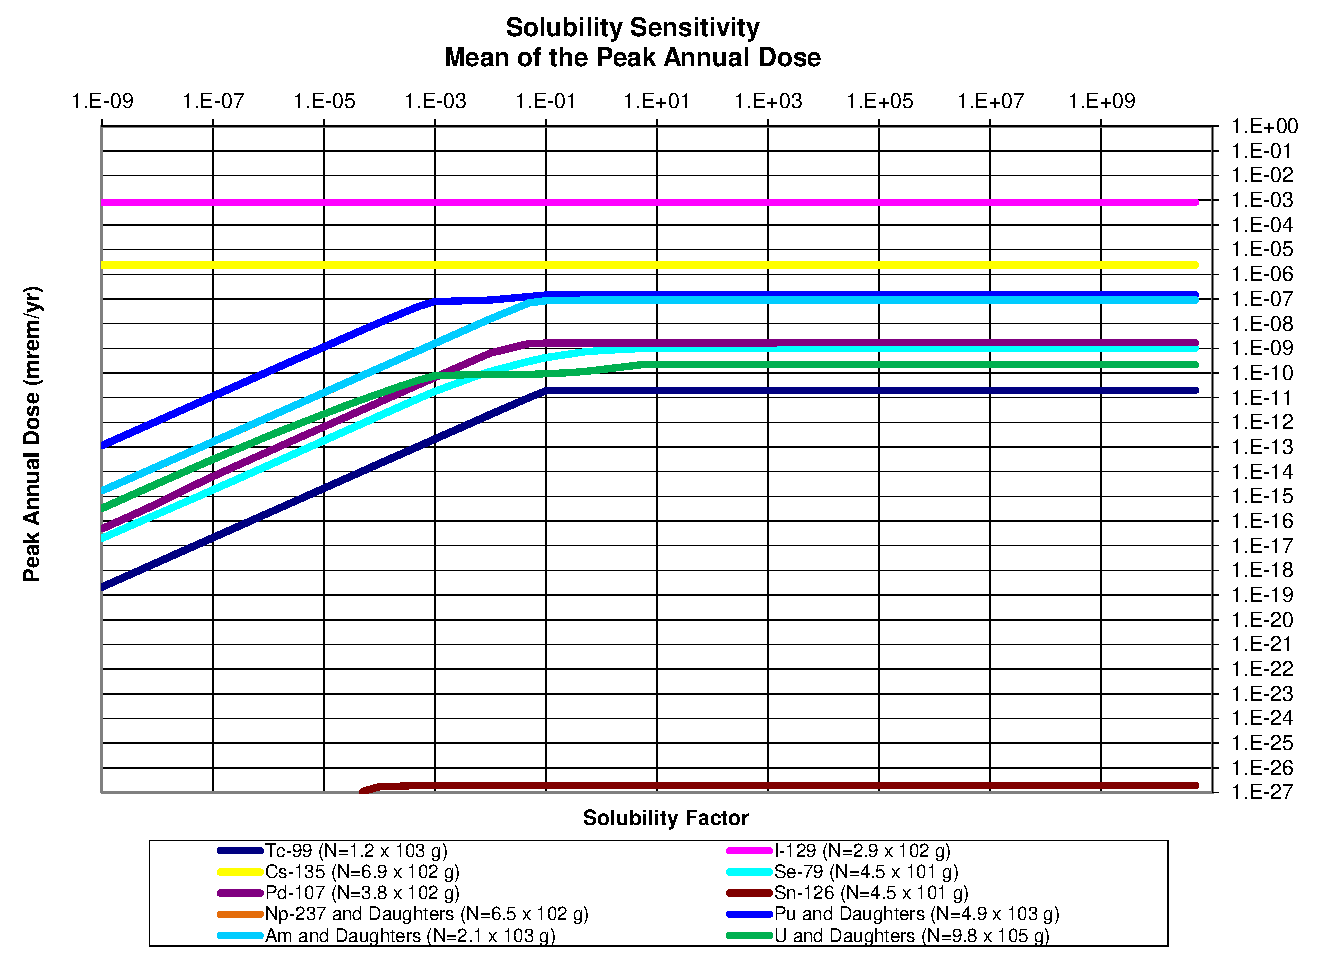
\includegraphics[width=\linewidth]{./chapters/nuclide_sensitivity/clay/Solubility/Solubility_Summary_SolFactor.eps}
\caption{Solubility factor sensitivity. The peak annual dose due to an inventory, 
$N$, of each isotope.}
\label{fig:SolSumFactor}
\end{figure}

\begin{figure}[ht]
\centering
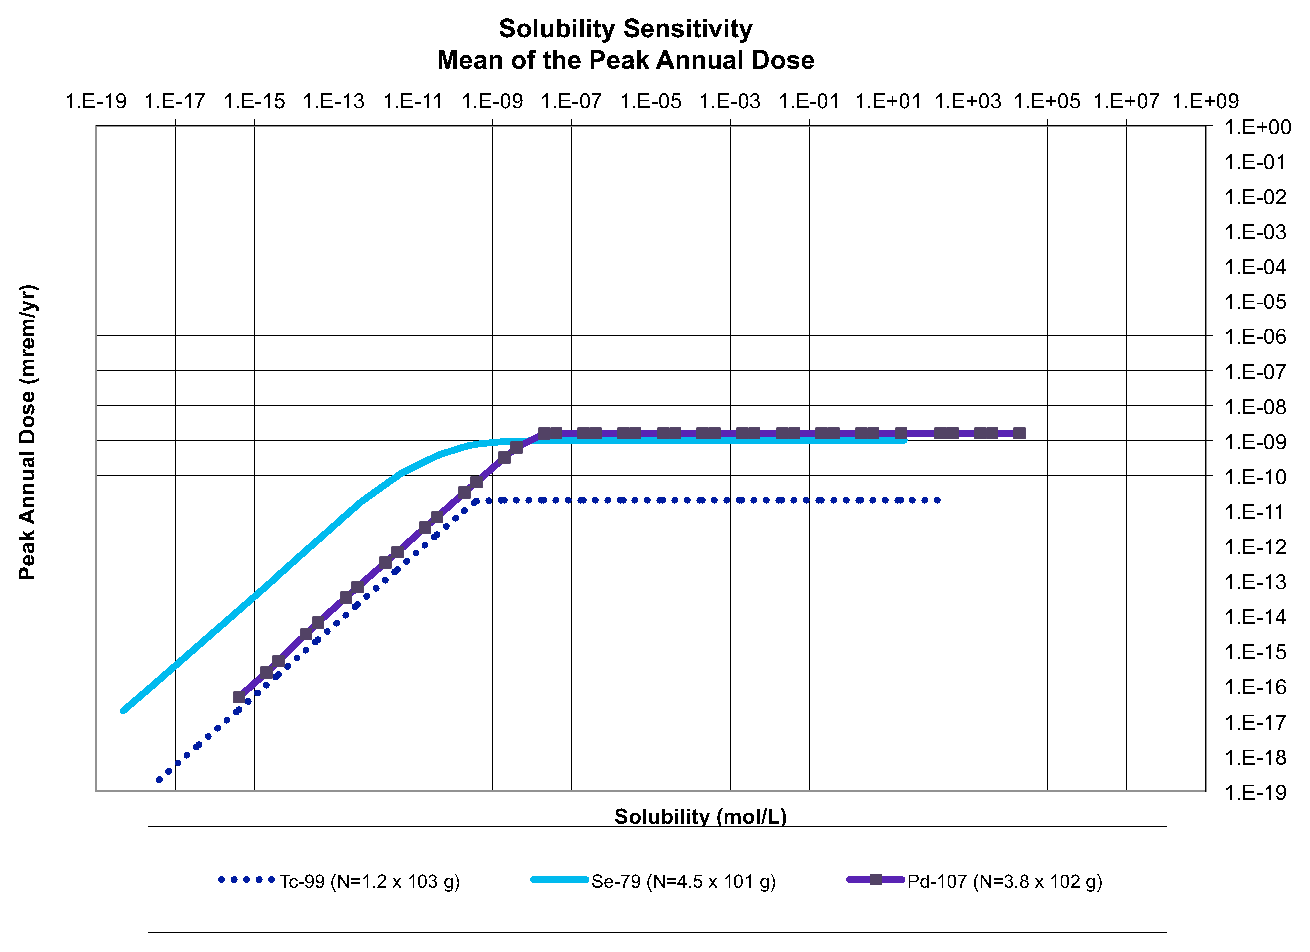
\includegraphics[width=\linewidth]{./chapters/nuclide_sensitivity/clay/Solubility/Solubility_Summary_Sol.eps}
\caption{Solubility limit sensitivity. The peak annual dose due to an inventory, 
$N$, of each isotope.}
\label{fig:SolSum}
\end{figure}
\clearpage


%\input{./chapters/sensitivity/wfdegradation}
%\input{./chapters/sensitivity/diffcoeff}
%\input{./chapters/sensitivity/advvec}
%\input{./chapters/sensitivity/wpfail}
%\input{./chapters/sensitivity/retardation}
%\input{./chapters/sensitivity/pathlength}

